\documentclass{article}
\title{\LaTeX Math notes}
\author{Samuel Hautamäki}
\date{th of October 2024}
\usepackage{mathtools,amssymb,amsthm,gensymb,textcomp}
\usepackage{graphicx}
\begin{document}
  \maketitle
   
  \section{Logarithmic function}
  HL p 477\\
  $y=a^x$ exponential eq\\
  $\Leftarrow\Rightarrow x=log_a(y)$\\
  $f(x)=a^x$, $f^{-1}(x)=log_a(x)$\\

  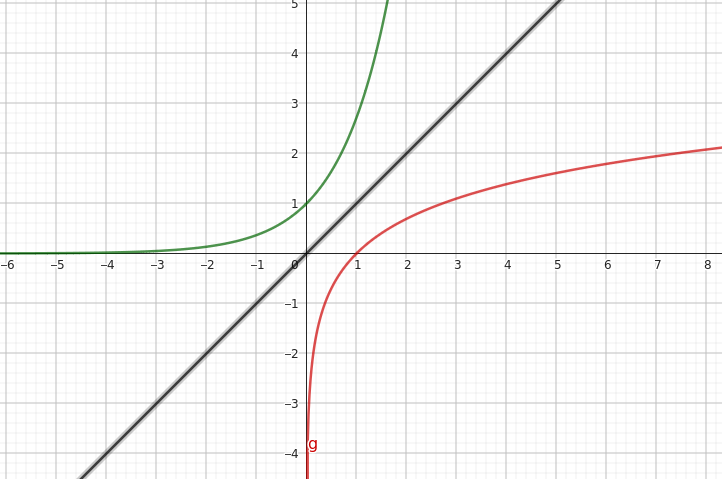
\includegraphics{log_exp_graph}

  All lograrithmic functions passes point (1,0)\\
  domain: $x>0$\\
  $range y\in\mathbb{R} ]-\infty,\infty[$\\
  $asymptote: y-axis, taht is x=0$\\
  functions are continuous(=jatkuva)\\
  if base $a>1$ of $f(x)=log_a(x)$ then increases.\\
  if base $0<a<1$ then decreasing\\
  if $a=1$ then $f(x)=constant$ horizontal line.\\
  Example.\\
  a) Sketch the Brigg's lograithm $f(x)=log_{10}(x)=lg(x)$\\
  base 10 means increasing, log passes (1,0), asymptote y-axis.\\
  b) Sketch the natural logaritmh, means base e.\\
  $f(x)=log_e(x)=ln(x)$\\
  pases point $(e,1)$\\
  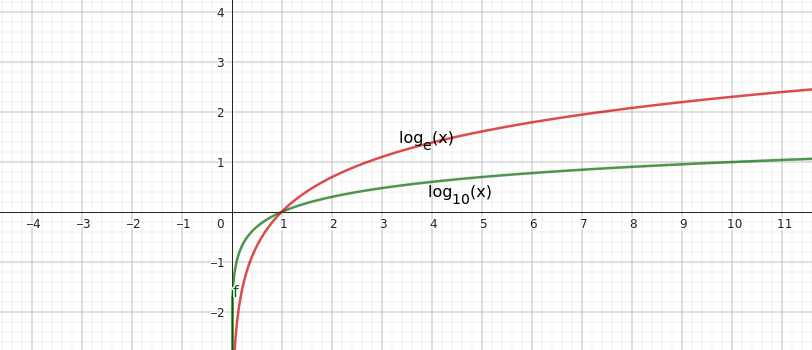
\includegraphics{log10e}
  \subsection{copy 9f}
  1a. $g(x)=log_3(x)+4$ has transmorfations of $f(x)=log_3(x)$\\
  Ans: 4 units.\\
  b) $h(x)=log_3(x-3)$\\
  Ans: 3 units to right\\
  c) $i(x)=2\cdot log_3(x)$ Ans: Stretch by 2 $y-axis\cdot2$\\
  9g 
  1.write in exponential form\\
  a. $log_p(q)=r \Leftarrow\Rightarrow p^r=q$\\
  see formula booklet 1.3\\
  b) $log_3(5)=r \Leftarrow\Rightarrow 3^r=5$\\
  c) $log_7(q)=6 == 7^6=q$\\
  d) $log_p(5)=3 == p^3=5$\\
  e) $log_1(1)=x == 1^x=1$\\
  2. \\
  a $r^s=t == log_r^t=s$\\ 
  b $8^2=64 == log_8(64)=2$\\
  c $10^x=25 == log_{10}^{25}=x$\\
  d $3^{-2}=\frac{1}{9}=log_3\frac{1}{9}=-2$\\

   
\end{document}
